\documentclass[leqno]{article}
% Shared mark scheme preamble for resources.danieljsmith.org: the pack
% preamble, unchanged, then the scheme's own layer. A scheme's .tex is
% rendered from its YAML (scripts/README.md, Mark schemes), never edited.
\input{\CurrentFilePath/pack_preamble.tex}

% The page: equal side margins, so the table runs the full width of the
% header rule. The footers' right edge follows the text's.
\geometry{left=0.8in, right=0.8in}
\makeatletter
\renewcommand{\djs@footR}[1]{%
  \put(\dimexpr1in+\hoffset+\oddsidemargin+\textwidth\relax,
    -\dimexpr\paperheight-0.32in\relax){\makebox[0pt][r]{#1}}}
\makeatother

\usepackage[export]{adjustbox}
\usepackage{tabularray}
\definecolor{msGrid}{RGB}{176, 172, 164}
\definecolor{msTint}{RGB}{245, 243, 239}

% The header on every page, the front page included, and the booklet label
% under the contents-page title. \djsQuestionPageStyle stays empty.
\newcommand{\djsSchemeHeader}[1]{%
  \djsPackHeader[markscheme]{\textit{Mark scheme} - #1}%
  \renewcommand{\djsPackTitle}{#1}%
  \renewcommand{\djsBookletLabel}{Mark scheme}%
}

% The front page: the contents heading, spaced as tocloft spaces the packs'
% "Questions", then the contents table. A question's name and page number
% both link to its first page.
\newcommand{\msContentsHeading}{%
  \vskip\cftbeforetoctitleskip
  {\noindent\cfttoctitlefont\contentsname\par}%
  \vskip\cftaftertoctitleskip}
\NewTblrEnviron{mscontents}
\SetTblrInner[mscontents]{
  colspec = {Q[wd=26mm, l] X[l] Q[wd=16mm, c] Q[wd=14mm, r]},
  width = \linewidth,
  rowsep = 4pt, colsep = 6pt,
  hlines = {0.4pt, msGrid}, vlines = {0.4pt, msGrid},
  hline{2} = {2.2pt, scarlet},
  row{1} = {font=\small\bfseries},
  row{Z} = {font=\bfseries},
  column{2} = {font=\small},
}
\newcommand{\msContentsQuestion}[1]{\hyperref[q:#1]{Question #1}}
\newcommand{\msContentsPage}[1]{\hyperref[q:#1]{\pageref*{q:#1}}}
\newcommand{\msSep}{\hspace{0.9em}}

% The conventions pages' layout: headings in the documents' own bold, tables
% ruled and padded as the scheme's, roomy lists.
\newcommand{\msHead}[1]{%
  \par\vspace{18pt}%
  {\noindent\bfseries #1\par}%
  \vspace{6pt}}
\NewTblrEnviron{mstblr}
\SetTblrInner[mstblr]{rowsep = 6pt, colsep = 6pt,
  hlines = {0.4pt, msGrid}, vlines = {0.4pt, msGrid}}
\newenvironment{msList}
  {\begin{itemize}[leftmargin=1.2em, itemsep=5pt, topsep=3pt, parsep=0pt]}
  {\end{itemize}}

% A question's first page: the link target and the PDF bookmark, as
% \questionitem gives the packs.
\newcommand{\msQnum}{}
\newcommand{\msQuestion}[1]{%
  \clearpage
  \renewcommand{\msQnum}{#1}%
  \phantomsection\label{q:#1}%
  \addcontentsline{toc}{subsection}{\protect\djsTocEntry{#1}}}

% The scheme's table: Question 16mm, Scheme the rest, Marks 16mm, Notes
% 44mm; every cell ruled in msGrid; the scarlet rule under the head row. A
% long table has no caption or "continued" foot; a continuation page opens
% with a muted line above the repeated head row. The rules across a part's
% rows, the alternative's tint and the total row are the rendered table's.
\NewTblrTheme{ms}{%
  \DefTblrTemplate{firsthead}{default}{}%
  \DefTblrTemplate{middlehead,lasthead}{default}{%
    {\small\itshape\color{djsMuted}Question \msQnum\ continued\par}%
    \vspace{6pt}}%
  \DefTblrTemplate{firstfoot,middlefoot,lastfoot}{default}{}%
}
\NewTblrEnviron{msscheme}
\SetTblrOuter[msscheme]{long, theme=ms, entry=none, label=none}
\SetTblrInner[msscheme]{
  colspec = {Q[wd=16mm, l] X[l] Q[wd=16mm, c] Q[wd=44mm, l]},
  width = \linewidth,
  rowsep = 6pt, colsep = 6pt,
  rowhead = 1,
  vlines = {0.4pt, msGrid},
  hline{1} = {0.4pt, msGrid}, hline{2} = {2.2pt, scarlet},
  hline{Z} = {0.4pt, msGrid},
  column{1} = {font=\bfseries}, column{3} = {font=\bfseries},
  column{4} = {font=\small},
  row{1} = {rowsep=4pt, font=\small\bfseries},
}

% Two marks on a row: each note starts with its code.
\newcommand{\msNote}[2]{\textbf{#1}\enspace #2}
% A full-row figure: the worked solution's own picture, scaled uniformly and
% only down, to the table less the Question column. The picture is drawn
% with the line width it has in the solutions document, at its list depth
% there (the optional argument, 1 by default: a part's working), so one
% sized by \linewidth keeps its size; tabularray sets the cell's \linewidth
% to the cell's measured width, which would shrink it at every pass. The
% widths are measured once, in a solution box at the packs' text width
% (pack_preamble.tex's margins, 0.8in and 1in).
\newlength{\msSpanW}
\makeatletter
\newcommand{\ms@keepLW}[1]{%
  \expandafter\xdef\csname ms@solnLW@#1\endcsname{\the\linewidth}}
\AtBeginDocument{%
  \setlength{\msSpanW}{\dimexpr\textwidth-16mm-28pt\relax}%
  \setbox\z@\vbox{%
    \begin{minipage}{\dimexpr\paperwidth-1.8in\relax}
      \begin{djsSolution}
        \ms@keepLW{0}%
        \begin{enumerate}\item \ms@keepLW{1}%
        \begin{enumerate}\item \ms@keepLW{2}%
        \begin{enumerate}\item \ms@keepLW{3}%
        \end{enumerate}\end{enumerate}\end{enumerate}
      \end{djsSolution}
    \end{minipage}}}
\newcommand{\msFigure}[2][1]{%
  \adjustbox{max width=\msSpanW, max totalheight=0.6\textheight, valign=t}{%
    \hsize=\csname ms@solnLW@#1\endcsname
    \linewidth=\hsize
    #2}}
\makeatother
% A figure mark's feature, in the Scheme column.
\newcommand{\msFeature}[1]{\textit{#1}}
% An alternative's title row.
\newcommand{\msAlternative}[1]{\textit{Alternative:} #1}
% Drafts only: a queried mark's code, the query's why under its note, and a
% flag in its part's place.
\newcommand{\msQueried}[2]{#1~\(\to\) #2?}
\newcommand{\msQuery}[1]{{\itshape\color{djsMuted}Query: #1}}
\newcommand{\msFlag}[2]{\textbf{#1:}\enspace #2}


\djsSchemeHeader{Rational Functions}
\djsSitePath{Core Pure}{Miscellaneous Pure}

\djsLastUpdated{29 October 2026}
\begin{document}
\djsSetQuestionCount{14}
\djsAddMarks{1}{8}
\djsAddMarks{2}{10}
\djsAddMarks{3}{9}
\djsAddMarks{4}{9}
\djsAddMarks{5}{12}
\djsAddMarks{6}{14}
\djsAddMarks{7}{14}
\djsAddMarks{8}{15}
\djsAddMarks{9}{12}
\djsAddMarks{10}{15}
\djsAddMarks{11}{15}
\djsAddMarks{12}{16}
\djsAddMarks{13}{14}
\djsAddMarks{14}{14}
\vspace*{6pt}
\djsContentsTitle
\vspace{30pt}
\msContentsHeading
\begin{mscontents}{}
Question & Marks by part & Marks & Page \\
\msContentsQuestion{1} & (a)\,1\msSep (b)\,2\msSep (c)\,1\msSep (d)\,4 & 8 & \msContentsPage{1} \\
\msContentsQuestion{2} & (a)\,2\msSep (b)\,3\msSep (c)\,2\msSep (d)\,3 & 10 & \msContentsPage{2} \\
\msContentsQuestion{3} & (a)\,2\msSep (b)\,5\msSep (c)\,2 & 9 & \msContentsPage{3} \\
\msContentsQuestion{4} & (a)(i)\,2\msSep (a)(ii)\,4\msSep (b)\,3 & 9 & \msContentsPage{4} \\
\msContentsQuestion{5} & (a)\,2\msSep (b)\,3\msSep (c)(i)\,3\msSep (c)(ii)\,4 & 12 & \msContentsPage{5} \\
\msContentsQuestion{6} & (a)\,5\msSep (b)\,3\msSep (c)\,2\msSep (d)\,4 & 14 & \msContentsPage{6} \\
\msContentsQuestion{7} & (a)\,1\msSep (b)\,4\msSep (c)\,3\msSep (d)(i)\,4\msSep (d)(ii)\,2 & 14 & \msContentsPage{7} \\
\msContentsQuestion{8} & (a)\,3\msSep (b)\,5\msSep (c)\,2\msSep (d)(i)\,4\msSep (d)(ii)\,1 & 15 & \msContentsPage{8} \\
\msContentsQuestion{9} & (a)\,3\msSep (b)\,4\msSep (c)\,3\msSep (d)\,2 & 12 & \msContentsPage{9} \\
\msContentsQuestion{10} & (a)\,3\msSep (b)\,4\msSep (c)\,3\msSep (d)(i)\,2\msSep (d)(ii)\,1\msSep (d)(iii)\,2 & 15 & \msContentsPage{10} \\
\msContentsQuestion{11} & (a)\,3\msSep (b)\,4\msSep (c)\,3\msSep (d)\,5 & 15 & \msContentsPage{11} \\
\msContentsQuestion{12} & (a)\,3\msSep (b)\,4\msSep (c)\,3\msSep (d)\,2\msSep (e)\,4 & 16 & \msContentsPage{12} \\
\msContentsQuestion{13} & (a)\,2\msSep (b)\,4\msSep (c)\,3\msSep (d)\,5 & 14 & \msContentsPage{13} \\
\msContentsQuestion{14} & (a)\,2\msSep (b)(i)\,4\msSep (b)(ii)\,3\msSep (c)\,5 & 14 & \msContentsPage{14} \\
\SetCell[c=2]{r} Total & & 177 & \\
\end{mscontents}
\newpage
% The conventions pages, shared by every pack's mark scheme: one source of
% truth, \input after the front page, with no strand or pack logic. The keys
% on the first side, the rules on the second. The scheme layer defines
% \msHead, msList and mstblr.
\vspace*{6pt}%
{\noindent\cfttoctitlefont Reading the mark scheme\par}%
\vspace{10pt}%
These rules apply throughout, unless a note says otherwise.

\msHead{Marks}
Every mark is worth one, so \textbf{M1 A1} on a row is two marks. Only marks
coded ft follow through.\par
\vspace{10pt}%
\begin{mstblr}{
  colspec = {Q[wd=15mm, l] X[l]},
  width = \linewidth,
  hline{2} = {2.2pt, scarlet},
  column{1} = {font=\bfseries},
  row{1} = {font=\small\bfseries, rowsep=4pt},
}
Code & Meaning \\
M1 & Method: a correct method, applied to this question. A slip doesn't cost it if the method is clear. A formula must be used, not just quoted. \\
dM1 & Dependent method: as M1, but only if the method mark before it was earned, unless its note names another. \\
A1 & Accuracy: a correct answer or step. It needs the method mark it follows. \\
A1ft & As A1, following through from an earlier answer that the note names. \\
A1~AG & The last mark of a part whose answer is printed in the question: complete working, with no errors. \\
B1 & A correct value, fact or statement. It needs no method mark. \\
B1ft & As B1, following through from an earlier answer that the note names. \\
E1 & A written explanation, interpretation or conclusion. Concluding a proof by induction needs every earlier mark. \\
\end{mstblr}

\msHead{Abbreviations}
ft and AG qualify a code in the Marks column. The others appear in the
notes.\par
\vspace{10pt}%
\begin{mstblr}{
  colspec = {Q[wd=17mm, l] X[l] Q[wd=15mm, l] X[l]},
  width = \linewidth,
  column{1} = {font=\bfseries}, column{3} = {font=\bfseries},
}
ft & follow through & AG & answer given in the question \\
cao & correct answer only, with no follow-through & cso & correct solution only: no errors in the part \\
oe & or an equivalent form & awrt & any answer that rounds to this value \\
soi & seen, or implied by later working & isw & ignore working after a correct answer \\
SC & special case: credit outside the main method & their & the student's own earlier value \\
condone & a slip that doesn't cost the mark & [\;\,] & working the mark doesn't need \\
s.f. & significant figures & d.p. & decimal places \\
\end{mstblr}

\newpage
\msHead{Reading the scheme}
\begin{msList}
\item Each row is a line of working, with the marks it earns beside it.
  Where a row carries two marks, each note starts with its code.
\item \textbf{[\textit{n}]} ends each part with its total.
\item A shaded \textit{Alternative} is a second method for the same total.
  Mark an answer by the method it follows.
\item Any other valid method earns the equivalent marks, unless the question
  names a method or says \textit{hence}.
\item A sketch earns one B1 for each feature named below its figure.
\end{msList}

\msHead{Accuracy and answers}
\begin{msList}
\item Unless a question says otherwise, give answers to 3 significant
  figures, and angles in degrees to 1 decimal place. Angles in radians take
  3 significant figures.
\item A final answer with more figures is accepted if it rounds to the
  scheme's value; one with fewer is not. An answer spoiled by rounding too
  early loses its accuracy mark.
\item Where a question asks for an exact answer, a decimal loses the final
  accuracy mark. Otherwise either is accepted.
\item Wrong or missing units cost nothing unless the question asks for them.
\item A correct answer with no working earns full marks, unless the question
  needs the working: show that, prove, hence, a method it names, or an exact
  answer. A wrong answer with no working earns nothing. Calculator answers
  are treated the same way.
\item A correct answer, once reached, isn't spoiled by later working (isw).
\end{msList}

\msHead{Value of $\boldsymbol{g}$}
\begin{msList}
\item Take $g = 9.8\,\mathrm{m\,s^{-2}}$ unless a question states a value,
  which is then the only one accepted. Answers that use $g = 9.8$ may be
  given to 2 or 3 significant figures.
\item Where a question doesn't state $g$, an answer worked with $g = 10$
  throughout earns the same marks, keeping any value printed in the
  question. The worked solutions list the final answers with $g = 10$.
\end{msList}


\msQuestion{1}
\begin{msscheme}{
  hline{3,5-6,8,10-13} = {2-Z}{0.4pt, msGrid},
  hline{4,7,9,14} = {0.4pt, msGrid},
  row{14} = {font=\bfseries},
}
Question & Scheme & Marks & Notes \\
1(a) & {\(y = 5\)} & B1 & \\
\nopagebreak & & [1] & \\
1(b) & {\(x^2 + bx + a = (x+1)(x-2) = x^2 - x - 2\)} & M1 & {Compares coefficients of \(x^2+bx+a\) with \((x+1)(x-2)\), or substitutes \(x=-1\) and \(x=2\) into \(x^2+bx+a=0\) and solves. Condone sign slips.} \\
& {\(a = -2,\ b = -1\)} & A1 & {Both values.} \\
\nopagebreak & & [2] & \\
1(c) & {\(\left(0, -\tfrac12\right)\)} & B1 & {Accept \(y = -\frac12\) stated with \(x = 0\).} \\
\nopagebreak & & [1] & \\
1(d) & {\(5x^2 - 2x + 1 = 4(x^2 - x - 2)\)} & M1 & {Equates their curve to 4 and multiplies by the denominator, collecting to a three-term quadratic. Condone sign slips.} \\
& {\(x^2 + 2x + 9 = 0\)} & A1 & {oe, any nonzero multiple.} \\
& {\(2^2 - 4(1)(9) = \ldots\)} & M1 & {Evaluates \(b^2-4ac\) for their three-term quadratic, or completes the square. Condone a slip in the value.} \\
& {\(= -32 < 0 \Rightarrow\) no real roots, so \(y = 4\)\\[4pt] does not intersect \(C\)} & A1~AG & {\(-32<0\), or \((x+1)^2+8>0\), from the correct quadratic, with a conclusion that there are no real roots so no intersection.} \\
\nopagebreak & & [4] & \\
\nopagebreak \SetCell[c=2]{r} Total for Question 1 & & 8 & \\
\end{msscheme}

\msQuestion{2}
\begin{msscheme}{
  hline{3-4,6-9,11-12,14-16} = {2-Z}{0.4pt, msGrid},
  hline{5,10,13,17} = {0.4pt, msGrid},
  row{17} = {font=\bfseries},
}
Question & Scheme & Marks & Notes \\
2(a) & {\(x = -3\)} & B1 & \\
& {\(y = -2\)} & B1 & \\
\nopagebreak & & [2] & \\
2(b) & \SetCell[c=3]{c} \msFigure{\begin{tikzpicture}
\begin{axis}[
    axis lines=center,
    xlabel={$x$},
    ylabel={$y$},
    xmin=-10, xmax=10,
    ymin=-10, ymax=10,
    xtick={-3,3},
    ytick={-2,2},
    width=0.8\linewidth,
    height=8.5cm,
    clip=true,
    every axis x label/.style={at={(ticklabel* cs:1)}, anchor=west},
    every axis y label/.style={at={(ticklabel* cs:1)}, anchor=south west},
]
\addplot[dashed, black] coordinates {(-3,-10) (-3,10)};
\addplot[dashed, black] coordinates {(-10,-2) (10,-2)};
\addplot[thick, black, samples=200, domain=-10:-3.15] {-2 + 12/(x+3)};
\addplot[thick, black, samples=200, domain=-2.85:10] {-2 + 12/(x+3)};
\node[below left] at (axis cs:0,0) {$O$};
\node[fill=white, inner sep=1pt] at (axis cs:4.8,-0.6) {$C_1$};
\end{axis}
\end{tikzpicture}} & & \\
& \msFeature{Shape} & B1 & {Two branches in the upper-right and lower-left regions, approaching the asymptotes without crossing them.} \\
& \msFeature{Asymptotes} & B1 & {Both asymptotes drawn and labelled \(x=-3\), \(y=-2\); values on the axes accepted.} \\
& \msFeature{Intercepts} & B1 & {Both \((0,2)\) and \((3,0)\), marked or stated; values on the axes accepted.} \\
\nopagebreak & & [3] & \\
2(c) & {Critical values \(x = -3\), \(x = 3\)} & M1 & {Uses the vertical asymptote and their \(x\)-intercept as critical values, from the sketch or algebraically, e.g. multiplying by \((x+3)^2\).} \\
& {\(-3 < x < 3\)} & A1 & {oe, e.g. set notation. A0 for \(\leq\) at either end or any extra interval.} \\
\nopagebreak & & [2] & \\
2(d) & {\(-x = -2 + \frac{12}{-y+3}\)} & M1 & {Replaces \(x\) by \(-y\) and \(y\) by \(-x\) in the equation of \(C_1\). Not for swapping \(x\) and \(y\) without the sign changes.} \\
& {\(2 - x = \frac{12}{3-y}\)\\[4pt] \(\Rightarrow 3 - y = \frac{12}{2-x} \Rightarrow y = \ldots\)} & dM1 & {Rearranges their equation to make \(y\) the subject, clearing the fraction. Condone sign slips.} \\
& {\(y = 3 + \frac{12}{x-2}\)} & A1 & {cso. oe in the form \(y = f(x)\), e.g. \(y = \frac{3x+6}{x-2}\).} \\
\nopagebreak & & [3] & \\
\nopagebreak \SetCell[c=2]{r} Total for Question 2 & & 10 & \\
\end{msscheme}

\msQuestion{3}
\begin{msscheme}{
  hline{3-4,6-11,13-14} = {2-Z}{0.4pt, msGrid},
  hline{5,12,15} = {0.4pt, msGrid},
  row{15} = {font=\bfseries},
}
Question & Scheme & Marks & Notes \\
3(a) & {\(x = 2,\ x = -2\)} & B1 & {Both needed.} \\
& {\(y = 1\)} & B1 & \\
\nopagebreak & & [2] & \\
3(b) & \SetCell[c=3]{c} \msFigure{\begin{tikzpicture}
\begin{axis}[
  width=0.8\linewidth,
  height=8.5cm,
  axis lines=middle,
  xmin=-6, xmax=6,
  ymin=-6, ymax=8,
  xlabel={$x$},
  ylabel={$y$},
  xtick={-3,-2,2,3},
  ytick={1,2.25},
  xticklabels={,,,},
  yticklabels={,},
  samples=300,
  clip=true,
  every axis x label/.style={
    at={(current axis.right of origin)},
    anchor=west,
    xshift=0pt
  },
]
  \addplot[dashed] coordinates {(-2,-6) (-2,8)};
  \addplot[dashed] coordinates {(2,-6) (2,8)};
  \addplot[dashed] coordinates {(-6,1) (6,1)};
  \addplot[domain=-6:-2.03, smooth, thick] {(x^2-9)/(x^2-4)};
  \addplot[domain=-1.97:1.97, smooth, thick] {(x^2-9)/(x^2-4)};
  \addplot[domain=2.03:6, smooth, thick] {(x^2-9)/(x^2-4)};
  \node[below=2pt] at (axis cs:-3,0) {$-3$};
  \node[below=2pt, xshift=-8pt] at (axis cs:-1.4,0) {$-2$};
  \node[below=2pt, xshift=8pt] at (axis cs:1.4,0) {$2$};
  \node[below=2pt] at (axis cs:3,0) {$3$};
  \node[left=4pt, yshift=-1pt, fill=white, inner sep=1pt] at (axis cs:0,1) {$1$};
  \node[left=3pt, yshift=4pt, fill=white, inner sep=1pt] at (axis cs:0,2.7) {$\frac94$};
\end{axis}
\end{tikzpicture}} & & \\
& \msFeature{Shape} & B1 & {U-shaped branch between the vertical asymptotes, tending to \(+\infty\) at both, with its minimum on the positive \(y\)-axis.} \\
& \msFeature{Shape} & B1 & {Both outer branches rising from \(-\infty\) at the vertical asymptotes, crossing the \(x\)-axis and approaching \(y = 1\) from below.} \\
& \msFeature{Asymptotes} & B1 & {\(x = \pm 2\) and \(y = 1\) drawn, labelled by equations or values on the axes.} \\
& \msFeature{Intercepts} & B1 & {\((-3, 0)\) and \((3, 0)\) on the outer branches; values on the axis accepted.} \\
& \msFeature{Intercepts} & B1 & {\(\left(0, \frac94\right)\) or 2.25 marked on the central branch.} \\
\nopagebreak & & [5] & \\
3(c) & {Curve between \(y = 0\) and \(y = 1\):\\[4pt] critical values \(x = \pm 3\) \(\Rightarrow x \ldots\)} & M1 & {Uses their \(x\)-intercepts as critical values and identifies where the curve lies between \(y=0\) and \(y=1\), from the sketch or algebraically.} \\
& {\(x < -3\) or \(x > 3\)} & A1 & {oe, such as \(|x| > 3\) or set notation. Strict inequalities, with no other region.} \\
\nopagebreak & & [2] & \\
\nopagebreak \SetCell[c=2]{r} Total for Question 3 & & 9 & \\
\end{msscheme}

\msQuestion{4}
\begin{msscheme}{
  hline{3-4,6-10,12-14} = {2-Z}{0.4pt, msGrid},
  hline{5,11,15} = {0.4pt, msGrid},
  row{15} = {font=\bfseries},
}
Question & Scheme & Marks & Notes \\
4(a)(i) & {\(x = -2,\ x = 3\)} & B1 & {Both, and no other vertical asymptotes.} \\
& {\(y = 0\)} & B1 & \\
\nopagebreak & & [2] & \\
4(a)(ii) & \SetCell[c=3]{c} \msFigure[2]{\begin{tikzpicture}
\begin{axis}[
  width=0.78\linewidth,
  height=8.5cm,
  axis lines=middle,
  xmin=-6, xmax=6,
  ymin=-5, ymax=5,
  xlabel={$x$},
  ylabel={$y$},
  xtick={-2,1,3},
  ytick={0.1666667},
  yticklabels={$ \frac16 $},
  yticklabel style={xshift=1pt, yshift=9pt},
  every axis x label/.style={
    at={(current axis.right of origin)},
    anchor=west,
    xshift=3pt
  },
  clip=true
]
\addplot[thick, smooth, domain=-6:-2.05, samples=200] {(x-1)/(x^2-x-6)};
\addplot[thick, smooth, domain=-1.95:2.95, samples=200] {(x-1)/(x^2-x-6)};
\addplot[thick, smooth, domain=3.05:6, samples=200] {(x-1)/(x^2-x-6)};
\addplot[dashed] coordinates {(-2,-5) (-2,5)};
\addplot[dashed] coordinates {(3,-5) (3,5)};
\end{axis}
\end{tikzpicture}} & & \\
& \msFeature{Shape} & B1 & {Left branch below the \(x\)-axis, to \(-\infty\) at \(x=-2\) and to 0 as \(x \to -\infty\); right branch above, from \(+\infty\) at \(x=3\) to 0.} \\
& \msFeature{Shape} & B1 & {Decreasing from \(+\infty\) at \(x=-2\) to \(-\infty\) at \(x=3\), crossing the \(x\)-axis once.} \\
& \msFeature{Asymptotes} & B1 & {All three asymptotes shown: \(x=-2\), \(x=3\), \(y=0\), labelled by equations or values on the axes.} \\
& \msFeature{Intercepts} & B1 & {Both \((1,0)\) and \(\left(0,\frac16\right)\), marked or stated; values on the axes accepted.} \\
\nopagebreak & & [4] & \\
4(b) & {\(\frac{x-1}{x^2-x-6} = \frac12 \Rightarrow x^2 - 3x - 4 = 0\)\\[4pt] \(\phantom{\frac{x-1}{x^2-x-6}} \Rightarrow x = \ldots\)} & M1 & {Equates the curve to \(\frac12\), clears fractions to a three-term quadratic and solves it by any means. Condone sign slips in rearranging.} \\
& {\(x = -1,\ x = 4\)} & A1 & \\
& {\(-2 < x < -1\) or \(3 < x < 4\)} & A1 & {Both intervals with strict inequalities, oe in set notation; condone ``and'' between them. A0 if any extra interval is given.} \\
\nopagebreak & & [3] & \\
\nopagebreak \SetCell[c=2]{r} Total for Question 4 & & 9 & \\
\end{msscheme}

\msQuestion{5}
\begin{msscheme}{
  hline{3-4,6-8,10-11,13-16} = {2-Z}{0.4pt, msGrid},
  hline{5,9,12,17} = {0.4pt, msGrid},
  row{17} = {font=\bfseries},
}
Question & Scheme & Marks & Notes \\
5(a) & {\(y = 2\)} & B1 & {Must be an equation, not 2 alone.} \\
& {\(x = -1\)} & B1 & {Must be an equation, not \(-1\) alone.} \\
\nopagebreak & & [2] & \\
5(b) & {\(3x + c = 2 - \frac{3}{x+1}\)\\[4pt] \(\Rightarrow (3x + c - 2)(x+1) = -3\)} & M1 & {Equates line and curve and multiplies through by \(x+1\). Condone sign slips.} \\
& {\(3x^2 + 3x + (c-2)x + c - 2 = -3\)} & A1 & {Correct expanded equation with no fractions, any arrangement; terms need not be collected.} \\
& {\(3x^2 + (c+1)x + (c+1) = 0\)} & A1~AG & {From a correct expanded equation, reaches the printed result, including \(= 0\), with no errors; collected steps accepted.} \\
\nopagebreak & & [3] & \\
5(c)(i) & {\(b^2 - 4ac = 0\):\\[4pt] \((c+1)^2 - 12(c+1) = 0\)} & M1 A1 & {\msNote{M1}{Sets the discriminant of the quadratic in (b) to zero, with its coefficients substituted. Condone one slip. Not for a calculus method.}\\ \msNote{A1}{oe, e.g. \(c^2 - 10c - 11 = 0\).}} \\
& {\(c = -1\) or \(c = 11\)} & A1 & {Both values and no others.} \\
\nopagebreak & & [3] & \\
5(c)(ii) & {\(x = -\frac{c+1}{2 \times 3}\) with \(c = \their{-1}, \their{11}\)\\[4pt] \(\Rightarrow x = \ldots\)} & M1 & {Finds the repeated root for at least one of their values of \(c\), by \(x = -\frac{b}{2a}\) or by solving the quadratic in (b).} \\
& {\(x = 0\), \(x = -2\)} & A1 & {Both values.} \\
& {\(y = 3(0) - 1\), \(y = 3(-2) + 11\)} & dM1 & {Substitutes their \(x\) with its corresponding \(c\) into the line, or substitutes \(x\) into the curve, to find \(y\).} \\
& {\((0, -1)\) and \((-2, 5)\)} & A1 & {Both points, correctly paired.} \\
\nopagebreak & & [4] & \\
\nopagebreak \SetCell[c=2]{r} Total for Question 5 & & 12 & \\
\end{msscheme}

\msQuestion{6}
\begin{msscheme}{
  hline{3-7,9-15,17-18,20-24} = {2-Z}{0.4pt, msGrid},
  hline{8,16,19,25} = {0.4pt, msGrid},
  cell{11-14}{2-4} = {bg=msTint},
  row{25} = {font=\bfseries},
}
Question & Scheme & Marks & Notes \\
6(a) & {\(y(2x-3)=-2x^2+11x-20\)} & M1 & {Multiplies by \(2x-3\) and rearranges towards a quadratic in \(x\) with coefficients in \(y\). Condone sign slips.} \\
& {\(2x^2+(2y-11)x+(20-3y)=0\)} & A1 & {oe, terms collected.} \\
& {\((2y-11)^2-4(2)(20-3y)\geq 0\)} & M1 & {Applies \(b^2-4ac\) to their quadratic in \(x\), with \(\geq\), \(>\) or \(=\), giving a quadratic in \(y\). Condone sign slips.} \\
& {\(4y^2-20y-39\geq 0 \Rightarrow y=\ldots\ [= -\tfrac32,\ \tfrac{13}{2}]\)} & dM1 & {Solves their three-term quadratic in \(y\) for its critical values by any means, calculator allowed.} \\
& {\(f(x)\leq -\tfrac32\) or \(f(x)\geq \tfrac{13}{2}\)} & A1 & {Both non-strict inequalities, oe in set or interval notation; \(y\) for \(f(x)\) condoned. No check of endpoints or \(x=\frac32\) needed. Accept the range from a correct sketch in (d).} \\
\nopagebreak & & [5] & \\
6(b) & {\(f'(x)=-1+\frac{16}{(2x-3)^2}\)} & M1 & {Differentiates by the quotient rule or after dividing. Condone sign and coefficient slips.} \\
& {\(f'(x)=0\Rightarrow (2x-3)^2=16\Rightarrow x=\ldots\)\\[4pt] \(\Rightarrow y=\ldots\)} & dM1 & {Sets their derivative to zero, solves for \(x\) and substitutes at least one root to find \(y\).} \\
& {\(\left(-\tfrac12,\tfrac{13}{2}\right)\), \(\left(\tfrac72,-\tfrac32\right)\)} & A1 & {Both points, correctly paired.} \\
& \SetCell[c=3]{l} \msAlternative{Repeated roots from (a)} & & \\
\nopagebreak & {\(2x^2+(2y-11)x+(20-3y)=0\)\\[4pt] \(y=\tfrac{13}{2}\Rightarrow (2x+1)^2=0\)\\[4pt] \(y=-\tfrac32\Rightarrow (2x-7)^2=0\)} & M1 & {Substitutes the critical values from (a) into their quadratic in \(x\). Condone sign slips.} \\
& {\(x=-\tfrac12\) or \(x=\tfrac72\)\\[4pt] Attained range endpoints are extrema, hence stationary points.} & dM1 & {Solves for the repeated roots and identifies the attained range endpoints as differentiable extrema, hence stationary points.} \\
& {\(\left(-\tfrac12,\tfrac{13}{2}\right)\), \(\left(\tfrac72,-\tfrac32\right)\)} & A1 & {Both points, correctly paired.} \\
\nopagebreak & & [3] & \\
6(c) & {\(f(x)=-x+4-\frac{8}{2x-3}\)} & M1 & {Divides to the form \(ax+b+\frac{c}{2x-3}\) by any method; may be seen in (b). Condone arithmetic slips.} \\
& {\(y=-x+4\)} & A1 & {From a correct quotient; a slip in the remainder alone is condoned.} \\
\nopagebreak & & [2] & \\
6(d) & \SetCell[c=3]{c} \msFigure{\begin{tikzpicture}
\begin{axis}[
width=0.82\linewidth,
height=8.7cm,
axis lines=middle,
xmin=-4, xmax=8,
ymin=-12, ymax=15,
xlabel={$x$},
ylabel={$y$},
xtick=\empty,
ytick=\empty,
extra y ticks={6.6666667},
extra y tick labels={$\frac{20}{3}$},
every extra y tick/.style={
    yticklabel style={anchor=east, xshift=20pt, yshift=-8pt}
},
samples=300,
clip=true
]
\addplot[dashed,domain=-4:8] {-x+4};
\addplot[dashed] coordinates {(1.5,-12) (1.5,15)};
\addplot[thick,domain=-4:1.45] {(-2*x^2+11*x-20)/(2*x-3)};
\addplot[thick,domain=1.55:8] {(-2*x^2+11*x-20)/(2*x-3)};
\addplot[only marks,mark=*] coordinates {(-0.5,6.5) (3.5,-1.5)};
\node[fill=white, inner sep=1pt] at (axis cs:-1,8) {$\left(-\frac12,\frac{13}{2}\right)$};
\node[fill=white, inner sep=1pt] at (axis cs:4,-3) {$\left(\frac72,-\frac32\right)$};
\node[fill=white, inner sep=1pt] at (axis cs:-3.05,5.15) {$y=-x+4$};
\node[fill=white, inner sep=1pt] at (axis cs:2.1,13.8) {$x=\frac32$};
\end{axis}
\end{tikzpicture}} & & \\
& \msFeature{Shape} & B1 & {Left branch left of the vertical asymptote and above the oblique; right branch right of the vertical and below the oblique. Both approach the asymptotes, with no \(x\)-intercepts.} \\
& \msFeature{Asymptotes} & B1 & {Vertical asymptote at \(x=\frac32\), labelled.} \\
& \msFeature{Asymptotes} & B1 & {Oblique asymptote with negative gradient, labelled \(y=-x+4\).} \\
& \msFeature{Turning points} & B1 & {Both points labelled with coordinates: minimum \(\left(-\frac12,\frac{13}{2}\right)\) on the left branch, maximum \(\left(\frac72,-\frac32\right)\) on the right.} \\
\nopagebreak & & [4] & \\
\nopagebreak \SetCell[c=2]{r} Total for Question 6 & & 14 & \\
\end{msscheme}

\msQuestion{7}
\begin{msscheme}{
  hline{3,5-7,9-11,13-16,18-19} = {2-Z}{0.4pt, msGrid},
  hline{4,8,12,17,20} = {0.4pt, msGrid},
  row{20} = {font=\bfseries},
}
Question & Scheme & Marks & Notes \\
7(a) & {\(y = 1\)} & B1 & \\
\nopagebreak & & [1] & \\
7(b) & {\(p^2 - 4(1)(4) < 0 \Rightarrow p^2 - 16 < 0\)} & M1 A1 & {\msNote{M1}{Uses the discriminant of the denominator, set negative. Condone \(\leq\) for this mark.}\\ \msNote{A1}{\(p^2 - 16 < 0\) oe, such as \(p^2 < 16\).}} \\
& {\(p^2 = 16 \Rightarrow p = \ldots\), inside region} & dM1 & {Finds the critical values of their quadratic inequality and selects the inside region.} \\
& {\(-4 < p < 4\)} & A1 & {Strict inequalities; accept \(\{p : -4 < p < 4\}\) or \((-4, 4)\).} \\
\nopagebreak & & [4] & \\
7(c) & {\(x^2 + 2x - 3 = 0 \Rightarrow x = \ldots\)} & M1 & {Sets the numerator equal to zero and solves by any means.} \\
& {\((-3, 0)\), \((1, 0)\)} & A1 & {Both points, and no others.} \\
& {\(\left(0, -\tfrac34\right)\)} & B1 & \\
\nopagebreak & & [3] & \\
7(d)(i) & {\(x^2 + 2x - 3 = k(x^2 - x + 4)\)} & M1 & {Sets the curve equal to \(k\), clears the fraction and collects into a three-term quadratic in \(x\). Condone sign slips.} \\
& {\((1-k)x^2 + (2+k)x - (3+4k) = 0\)} & A1 & {Correct quadratic, oe with all terms on one side.} \\
& {\((2+k)^2 - 4(1-k)\bigl(-(3+4k)\bigr) \geq 0\)} & M1 & {Uses \(b^2 - 4ac\) with their coefficients in \(k\), set non-negative. Condone \(>\) or \(=\) for this mark.} \\
& {\(\Rightarrow -15k^2 + 8k + 16 \geq 0\)\\[4pt] \(\Rightarrow 15k^2 - 8k - 16 \leq 0\)} & A1~AG & {Correct substituted discriminant with \(\geq 0\), expanded without error to the printed result, the inequality reversed correctly on changing signs.} \\
\nopagebreak & & [4] & \\
7(d)(ii) & {\(15k^2 - 8k - 16 = 0 \Rightarrow k = \ldots\)} & M1 & {Solves \(15k^2 - 8k - 16 = 0\) by any means, calculator allowed.} \\
& {\(k = \tfrac43\) or \(-\tfrac45\)\\[4pt] \(y\)-coordinate of \(M\) is \(\tfrac43\)} & A1 & {\(\frac43\) or awrt 1.33 given as the answer; A0 if \(-\frac45\) is also given as the \(y\)-coordinate.} \\
\nopagebreak & & [2] & \\
\nopagebreak \SetCell[c=2]{r} Total for Question 7 & & 14 & \\
\end{msscheme}

\msQuestion{8}
\begin{msscheme}{
  hline{3-5,7-11,13-15,17-21,23} = {2-Z}{0.4pt, msGrid},
  hline{6,12,16,22,24} = {0.4pt, msGrid},
  row{24} = {font=\bfseries},
}
Question & Scheme & Marks & Notes \\
8(a) & {\(x = -1\)} & B1 & \\
& {\(\frac{x^2+3}{x+1} = x - 1 + \frac{4}{x+1}\)} & M1 & {Divides to the form \(x + p + \frac{q}{x+1}\) by any method. Condone slips in \(p\) and \(q\).} \\
& {\(y = x - 1\)} & A1 & \\
\nopagebreak & & [3] & \\
8(b) & {\(y(x+1) = x^2 + 3\)} & M1 & {Multiplies by \(x + 1\) and rearranges towards a quadratic in \(x\) with coefficients in \(y\). Condone sign slips.} \\
& {\(x^2 - yx + (3 - y) = 0\)} & A1 & {oe, any arrangement equated to zero.} \\
& {Real \(x\) needs \(b^2 - 4ac \geq 0\):\\[4pt] \((-y)^2 - 4(3 - y) \geq 0\)\\[4pt] \(\phantom{A} \Rightarrow y^2 + 4y - 12 \geq 0\)} & M1 & {Uses the discriminant of their quadratic in \(x\) to form a quadratic inequality or equation in \(y\). Condone slips and a wrong inequality sign.} \\
& {\((y + 6)(y - 2) \geq 0 \Rightarrow y = \ldots\ [= -6,\ 2]\)} & dM1 & {Solves their three-term quadratic in \(y\) by factorising, formula, completing the square or calculator.} \\
& {\(y \leq -6\) or \(y \geq 2\)\\[4pt] so no point on \(C\) with \(-6 < y < 2\)} & A1~AG & {cso: correct region from \(b^2 - 4ac \geq 0\), or discriminant \(< 0\) shown for \(-6 < y < 2\), with a conclusion in words. A0 for the region alone.} \\
\nopagebreak & & [5] & \\
8(c) & \SetCell[c=3]{c} \msFigure{\begin{tikzpicture}
\begin{axis}[
width=0.78\linewidth,
height=8.8cm,
axis lines=middle,
xmin=-8, xmax=6,
ymin=-10, ymax=10,
xlabel={$x$},
ylabel={$y$},
xtick={-1},
ytick=\empty,
samples=250,
clip=true
]
\addplot[dashed, domain=-8:6] {x-1};
\node[fill=white, inner sep=1pt] at (axis cs:3.7,1.5) {$y=x-1$};
\addplot[dashed] coordinates {(-1,-10) (-1,10)};
\addplot[thick, domain=-8:-1.05] {(x^2+3)/(x+1)};
\addplot[thick, domain=-0.95:6] {(x^2+3)/(x+1)};
\end{axis}
\end{tikzpicture}} & & \\
& \msFeature{Shape} & B1 & {Two branches approaching both asymptotes without crossing them; right branch above the \(x\)-axis, left branch below it.} \\
& \msFeature{Asymptotes} & B1 & {Both asymptotes drawn and labelled \(x=-1\), \(y=x-1\). Intercept and turning-point labels are optional.} \\
\nopagebreak & & [2] & \\
8(d)(i) & \SetCell[c=3]{c} \msFigure[2]{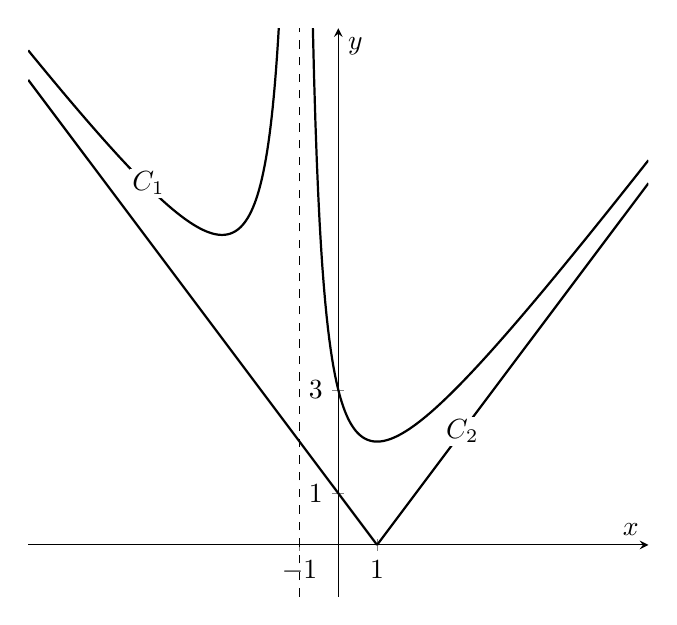
\begin{tikzpicture}
\begin{axis}[
width=0.78\linewidth,
height=8.8cm,
axis lines=middle,
xmin=-8, xmax=8,
ymin=-1, ymax=10,
xlabel={$x$},
ylabel={$y$},
xtick={-1,1},
ytick={1,3},
samples=250,
clip=true
]
\addplot[dashed] coordinates {(-1,-1) (-1,10)};
\addplot[thick, domain=-8:-1.05] {-(x^2+3)/(x+1)};
\addplot[thick, domain=-0.95:8] {(x^2+3)/(x+1)};
\addplot[thick, domain=-8:1] {1-x};
\addplot[thick, domain=1:8] {x-1};
\node[fill=white, inner sep=1pt] at (axis cs:-4.9,7) {$C_1$};
\node[fill=white, inner sep=1pt] at (axis cs:3.2,2.2) {$C_2$};
\end{axis}
\end{tikzpicture}} & & \\
& \msFeature{Shape} & B1 & {\(C_1\): right branch unchanged, left branch reflected above the \(x\)-axis; the whole curve is above the axis.} \\
& \msFeature{Asymptotes} & B1 & {\(C_1\) approaches \(x=-1\), \(y=1-x\) on the left and \(y=x-1\) on the right; \(C_2\) may supply the oblique asymptotes.} \\
& \msFeature{Shape} & B1 & {\(C_2\): V with vertex at \((1,0)\), arms of gradients \(-1\) and \(1\); \(C_1\) stays above it.} \\
& \msFeature{Intercepts} & B1 & {\((0,3)\) on \(C_1\), and both \((1,0)\), \((0,1)\) on \(C_2\), marked or stated; axis values accepted.} \\
\nopagebreak & & [4] & \\
8(d)(ii) & {\(c \leq 0\)} & B1 & {oe; the inequality must include 0.} \\
\nopagebreak & & [1] & \\
\nopagebreak \SetCell[c=2]{r} Total for Question 8 & & 15 & \\
\end{msscheme}

\msQuestion{9}
\begin{msscheme}{
  hline{3-9,11-13,15-18,20-22} = {2-Z}{0.4pt, msGrid},
  hline{10,14,19,23} = {0.4pt, msGrid},
  cell{5-8}{2-4} = {bg=msTint},
  row{23} = {font=\bfseries},
}
Question & Scheme & Marks & Notes \\
9(a) & {\(y=1\)} & B1 & \\
& {\((-2)^2-4(1)(3)=-8\)} & M1 & {Finds the discriminant of the denominator to examine whether it has real roots. Condone arithmetic slips.} \\
& {\(-8<0\Rightarrow\) denominator never zero\\[4pt] \(\Rightarrow\) no vertical asymptotes} & A1~AG & {Correct discriminant \(-8<0\) and conclusion that the denominator is never zero, hence no vertical asymptotes.} \\
& \SetCell[c=3]{l} \msAlternative{Completing the square} & & \\
\nopagebreak & {\(y=1\)} & B1 & \\
& {\(x^2-2x+3=(x-1)^2+2\)} & M1 & {Completes the square on the denominator to examine whether it has real roots.} \\
& {\((x-1)^2+2>0\) for all real \(x\)\\[4pt] \(\Rightarrow\) denominator never zero\\[4pt] \(\Rightarrow\) no vertical asymptotes} & A1~AG & {Correct positive square form for all real \(x\), with the conclusion that the denominator is never zero, hence no vertical asymptotes.} \\
\nopagebreak & & [3] & \\
9(b) & {\(\frac{\mathrm{d}y}{\mathrm{d}x}=\{(2x+2)(x^2-2x+3)\)\\[4pt] \(\phantom{=}-(x^2+2x-3)(2x-2)\}\div(x^2-2x+3)^2\)} & M1 A1 & {\msNote{M1}{Applies the quotient or product rule, with linear derivatives of numerator and denominator. Condone sign slips.}\\ \msNote{A1}{Any correct form, simplified or not.}} \\
& {\(12x-4x^2=0 \Rightarrow x=\ldots\)\\[4pt] \(\Rightarrow y=\ldots\)} & dM1 & {Sets their numerator equal to zero, solves by any method and substitutes at least one root into \(y\).} \\
& {\((0,-1)\) and \((3,2)\)} & A1 & {Both points and no others.} \\
\nopagebreak & & [4] & \\
9(c) & \SetCell[c=3]{c} \msFigure{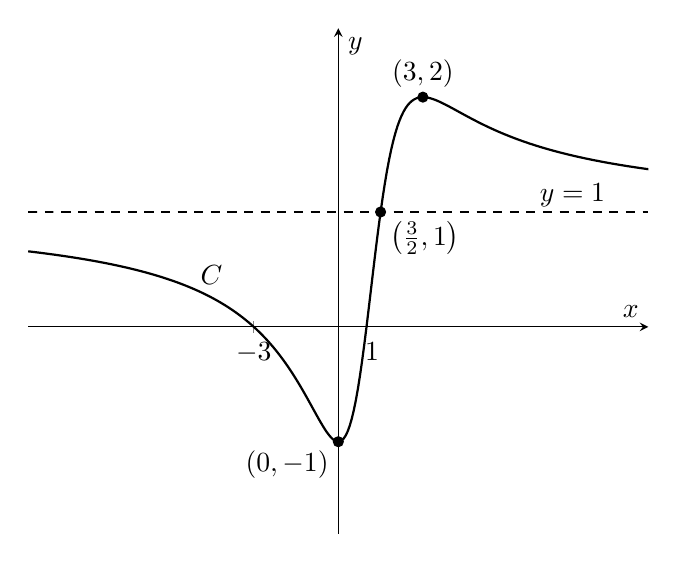
\begin{tikzpicture}
 \begin{axis}[
  width=0.78\linewidth,
  height=8cm,
  axis lines=middle,
  xlabel={$x$},
  ylabel={$y$},
  xmin=-11, xmax=11,
  ymin=-1.8, ymax=2.6,
  xtick={-3},
  xticklabels={$-3$},
  extra x ticks={1},
  extra x tick labels={$1$},
  extra x tick style={
    tick label style={xshift=2pt}
  },
  ytick=\empty,
  domain=-11:11,
  samples=300,
  clip=true
]
  \addplot[black, thick] {((x-1)*(x+3))/(x^2-2*x+3)};
  \addplot[black, dashed] {1};
  \addplot[only marks, mark=*, mark size=1.8pt] coordinates {(0,-1) (3,2) (1.5,1)};
  \node[left] at (axis cs:0,-1.2) {$(0,-1)$};
  \node[above] at (axis cs:3,2) {$(3,2)$};
  \node[below right] at (axis cs:1.5,1) {$\left(\frac32,1\right)$};
  \node[right] at (axis cs:6.8,1.15) {$y=1$};
  \node[fill=white, inner sep=1pt] at (axis cs:-4.5,0.45) {$C$};
  \end{axis}
  \end{tikzpicture}} & & \\
& \msFeature{Shape} & B1 & {One continuous curve: minimum on the negative \(y\)-axis, maximum in the first quadrant; both ends approach the horizontal asymptote, from below on the left and above on the right.} \\
& \msFeature{Asymptotes} & B1 & {Horizontal asymptote \(y=1\) drawn and labelled; \(1\) on the \(y\)-axis accepted.} \\
& \msFeature{Intercepts} & B1 & {All three \((-3,0)\), \((1,0)\), \((0,-1)\), marked or stated; values on the axes accepted.} \\
\nopagebreak & & [3] & \\
9(d) & \SetCell[c=3]{c} \msFigure{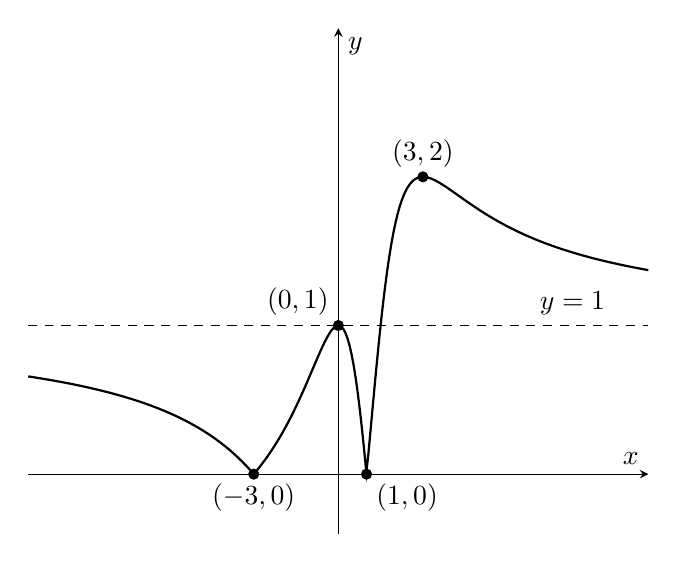
\begin{tikzpicture}
\begin{axis}[
width=0.78\linewidth,
height=8cm,
axis lines=middle,
xlabel={$x$},
ylabel={$y$},
xmin=-11, xmax=11,
ymin=-0.4, ymax=3,
xtick=\empty, ytick=\empty,
domain=-11:11,
samples=300,
clip=true
]
\addplot[black, thick] {abs(((x-1)*(x+3))/(x^2-2*x+3))};
\addplot[black, dashed] {1};
\addplot[only marks, mark=*, mark size=1.8pt] coordinates {(-3,0) (1,0) (0,1) (3,2)};
\node[below] at (axis cs:-3,0) {$(-3,0)$};
\node[below right] at (axis cs:1,0) {$(1,0)$};
\node[above left] at (axis cs:0,1) {$(0,1)$};
\node[above] at (axis cs:3,2) {$(3,2)$};
\node[right] at (axis cs:6.8,1.15) {$y=1$};
\end{axis}
\end{tikzpicture}} & & \\
& \msFeature{Shape} & B1 & {Part below the \(x\)-axis reflected above it, with cusps at \(x=-3\) and \(x=1\), and a local maximum on the positive \(y\)-axis.} \\
& {\(0<k<1\)} & B1 & {Strict inequalities, oe such as \(k\in(0,1)\).} \\
\nopagebreak & & [2] & \\
\nopagebreak \SetCell[c=2]{r} Total for Question 9 & & 12 & \\
\end{msscheme}

\msQuestion{10}
\begin{msscheme}{
  hline{3-5,7-10,12-15,17-19,21-22,24-25} = {2-Z}{0.4pt, msGrid},
  hline{6,11,16,20,23,26} = {0.4pt, msGrid},
  row{26} = {font=\bfseries},
}
Question & Scheme & Marks & Notes \\
10(a) & {\(x = -1\)} & B1 & \\
& {\(\frac{x^2+ax-6}{x+1} = x + \ldots + \frac{\ldots}{x+1}\)} & M1 & {Divides by \(x+1\) by any method, e.g. comparing coefficients, reaching a linear quotient \(x + \ldots\). Condone a wrong remainder.} \\
& {\(y = x + a - 1\)} & A1 & {Must be an equation; \(x + a - 1\) alone scores A0.} \\
\nopagebreak & & [3] & \\
10(b) & {\(y = x + a - 1 - (a+5)(x+1)^{-1}\)\\[4pt] \(\Rightarrow \frac{\mathrm{d}y}{\mathrm{d}x} = \ldots\)} & M1 & {Differentiates their (a) form with \((x+1)^{-1} \to k(x+1)^{-2}\), or the original by the quotient rule with denominator \((x+1)^2\). Condone sign slips.} \\
& {\(\frac{\mathrm{d}y}{\mathrm{d}x} = 1 + \frac{a+5}{(x+1)^2}\)} & A1 & {oe, e.g. \(\frac{x^2+2x+a+6}{(x+1)^2}\).} \\
& {\(a > 0 \Rightarrow \frac{a+5}{(x+1)^2} > 0\)} & dM1 & {Considers the sign of their derivative, or sets it to zero and tests for real roots, e.g. by discriminant or completing the square.} \\
& {\(\frac{\mathrm{d}y}{\mathrm{d}x} > 0\) for all \(x \ne -1\), so no stationary points} & A1~AG & {Correct derivative shown nonzero for all \(x\), using \(a>0\) or \(a+5>0\), with a conclusion in words. A0 without reference to \(a\).} \\
\nopagebreak & & [4] & \\
10(c) & \SetCell[c=3]{c} \msFigure{\begin{tikzpicture}
\def\a{3}
\begin{axis}[
  width=0.78\linewidth,
  height=8cm,
  axis lines=middle,
  xmin=-8, xmax=8,
  ymin=-10, ymax=10,
  xlabel={$x$},
  ylabel={$y$},
  xtick=\empty,
  ytick={-6},
  yticklabels={$-6$},
  yticklabel style={xshift=1pt, yshift=1pt},
  every axis x label/.style={
    at={(current axis.right of origin)},
    anchor=west,
    xshift=0pt
  },
  samples=300,
  clip=true,
  restrict y to domain=-10:10,
  unbounded coords=jump
]
  \addplot[dashed, domain=-8:8] {x + \a - 1};
  \addplot[dashed] coordinates {(-1,-10) (-1,10)};
  \addplot[thick, domain=-8:-1.03, smooth] {(x^2 + \a*x - 6)/(x + 1)};
  \addplot[thick, domain=-0.97:8, smooth] {(x^2 + \a*x - 6)/(x + 1)};
  \node[fill=white, inner sep=1pt] at (axis cs:-1,5) {$x=-1$};
  \node[fill=white, inner sep=1pt] at (axis cs:3.9,8.3) {$y=x+a-1$};
\end{axis}
\end{tikzpicture}} & & \\
& \msFeature{Shape} & B1 & {Two increasing branches, left above and right below the oblique asymptote, approaching both asymptotes, each crossing the \(x\)-axis once.} \\
& \msFeature{Asymptotes} & B1 & {Both asymptotes drawn and labelled \(x=-1\) and \(y = x + a - 1\).} \\
& \msFeature{Intercepts} & B1 & {\((0,-6)\) stated, or \(-6\) marked on the \(y\)-axis.} \\
\nopagebreak & & [3] & \\
10(d)(i) & \SetCell[c=3]{c} \msFigure[2]{\begin{tikzpicture}
\def\a{3}
\begin{axis}[
  width=0.78\linewidth,
  height=8cm,
  axis lines=middle,
  xmin=-8, xmax=8,
  ymin=-0.5, ymax=10,
  xlabel={$x$},
  ylabel={$y$},
  xtick={-1},
  xticklabels={$-1$},
  ytick=\empty,
  every axis x label/.style={
    at={(current axis.right of origin)},
    anchor=west,
    xshift=0pt
  },
  samples=300,
  clip=true,
  restrict y to domain=-0.5:10,
  unbounded coords=jump
]
  \addplot[dashed] coordinates {(-1,-0.5) (-1,10)};
  \addplot[thick, domain=-8:-1.03] {abs((x^2 + \a*x - 6)/(x + 1))};
  \addplot[thick, domain=-0.97:8]  {abs((x^2 + \a*x - 6)/(x + 1))};
\end{axis}
\end{tikzpicture}} & & \\
& \msFeature{Shape} & B1 & {Parts of \(C\) below the \(x\)-axis reflected above it; both branches tend to \(+\infty\) at \(x=-1\), with both ends rising.} \\
& \msFeature{Intercepts} & B1 & {Cusps on the \(x\)-axis, one on each side of \(x=-1\).} \\
\nopagebreak & & [2] & \\
10(d)(ii) & \SetCell[c=3]{c} \msFigure[2]{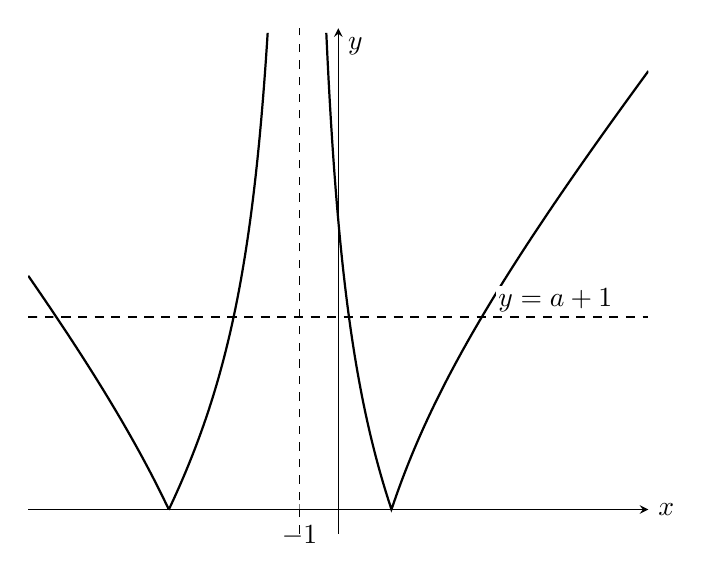
\begin{tikzpicture}
\def\a{3}
\begin{axis}[
  width=0.78\linewidth,
  height=8cm,
  axis lines=middle,
  xmin=-8, xmax=8,
  ymin=-0.5, ymax=10,
  xlabel={$x$},
  ylabel={$y$},
  xtick={-1},
  xticklabels={$-1$},
  ytick=\empty,
  every axis x label/.style={
    at={(current axis.right of origin)},
    anchor=west,
    xshift=0pt
  },
  samples=300,
  clip=true,
  restrict y to domain=-0.5:10,
  unbounded coords=jump
]
  \addplot[dashed] coordinates {(-1,-0.5) (-1,10)};
  \addplot[thick, domain=-8:-1.03] {abs((x^2 + \a*x - 6)/(x + 1))};
  \addplot[thick, domain=-0.97:8]  {abs((x^2 + \a*x - 6)/(x + 1))};
  \addplot[dashed, domain=-8:8] {\a + 1};
  \node[fill=white, inner sep=1pt] at (axis cs:5.6,4.35) {$y=a+1$};
\end{axis}
\end{tikzpicture}} & & \\
& \msFeature{Intercepts} & B1 & {Horizontal line meeting the curve four times, twice on each side of \(x=-1\).} \\
\nopagebreak & & [1] & \\
10(d)(iii) & {\(x = 0\) is a boundary:\\[4pt] \(\left|\frac{-6}{1}\right| = a + 1 \Rightarrow a = \ldots\)} & M1 & {Substitutes an endpoint of an interval, e.g. \(x = 0\), into \(\left|\frac{x^2+ax-6}{x+1}\right| = a+1\) and solves for \(a\).} \\
& {\(a = 5\)} & A1 & {\(a = 5\) only, with any other root from the modulus rejected.} \\
\nopagebreak & & [2] & \\
\nopagebreak \SetCell[c=2]{r} Total for Question 10 & & 15 & \\
\end{msscheme}

\msQuestion{11}
\begin{msscheme}{
  hline{3-5,7-9,11-14,16-28} = {2-Z}{0.4pt, msGrid},
  hline{6,10,15,29} = {0.4pt, msGrid},
  cell{21-27}{2-4} = {bg=msTint},
  row{29} = {font=\bfseries},
}
Question & Scheme & Marks & Notes \\
11(a) & {\(x=-2\)} & B1 & \\
& {\(x^2-6x+5=(x+2)(x+\ldots)+\ldots\)} & M1 & {Divides by \(x+2\) by any method to a quotient of the form \(x+k\). Condone an arithmetic slip in \(k\) or the remainder.} \\
& {\(y=x-8\)} & A1 & \\
\nopagebreak & & [3] & \\
11(b) & {\(\frac{\mathrm{d}y}{\mathrm{d}x}=1-\frac{21}{(x+2)^2}\)} & M1 A1 & {\msNote{M1}{Differentiates their divided form with \((x+2)^{-1}\to k(x+2)^{-2}\), or uses the quotient rule with numerator of the form \((x+2)(2x-6)\pm(x^2-6x+5)\).}\\ \msNote{A1}{oe, such as \(\frac{x^2+4x-17}{(x+2)^2}\).}} \\
& {\(1-\frac{21}{(x+2)^2}=0\Rightarrow x=\ldots\)\\[4pt] \(y=x-8+\frac{21}{x+2}\Rightarrow y=\ldots\)} & dM1 & {Sets their derivative to zero, solves for \(x\) by any method and substitutes at least one value into an equation of \(C\).} \\
& {\((-2-\sqrt{21},\,-10-2\sqrt{21})\)\\[4pt] \((-2+\sqrt{21},\,-10+2\sqrt{21})\)} & A1 & {Both points, exact and correctly paired, in any exact equivalent form.} \\
\nopagebreak & & [4] & \\
11(c) & \SetCell[c=3]{c} \msFigure{\begin{tikzpicture}
\begin{axis}[
  axis lines=middle,
  width=0.78\linewidth,
  height=8.5cm,
  xmin=-10, xmax=10,
  ymin=-35, ymax=25,
  xlabel={$x$},
  ylabel={$y$},
  xtick={1, 5},
  ytick={2.5},
  yticklabel={$\frac52$},
  enlargelimits=false,
  clip=true,
  every axis x label/.style={
  at={(current axis.right of origin)},
  anchor=west,
  xshift=0pt
},
]
  \addplot[domain=-10:-2.05, samples=300, smooth] {(x^2-6*x+5)/(x+2)};
  \addplot[domain=-1.95:10, samples=300, smooth] {(x^2-6*x+5)/(x+2)};
  \addplot[dashed, domain=-10:10] {x-8};
  \addplot[dashed] coordinates {(-2,-35) (-2,25)};
  \node[fill=white, inner sep=1pt] at (axis cs:-3.5,8) {$x=-2$};
  \node[fill=white, inner sep=1pt] at (axis cs:7,-3.5) {$y=x-8$};
  \node[fill=white, inner sep=1pt] at (axis cs:7,5) {$C$};
\end{axis}
\end{tikzpicture}} & & \\
& \msFeature{Shape} & B1 & {Two branches approaching both asymptotes: left branch with a maximum below the \(x\)-axis, right branch with a minimum below it.} \\
& \msFeature{Asymptotes} & B1 & {Both asymptotes drawn and labelled \(x=-2\), \(y=x-8\).} \\
& \msFeature{Intercepts} & B1 & {All three \((1,0)\), \((5,0)\), \(\left(0,\frac52\right)\), marked or stated; values on the axes accepted.} \\
\nopagebreak & & [3] & \\
11(d) & \SetCell[c=3]{c} \msFigure{\begin{tikzpicture}
\begin{axis}[
  axis lines=middle,
  width=0.78\linewidth,
  height=8.5cm,
  xmin=-10, xmax=10,
  ymin=-5, ymax=40,
  xlabel={$x$},
  ylabel={$y$},
  xtick={1, 5},
  ytick={2.5},
  yticklabel={$\frac52$},
  enlargelimits=false,
  clip=true,
  every axis x label/.style={
  at={(current axis.right of origin)},
  anchor=west,
  xshift=0pt
},
]
  \addplot[domain=-10:-2.05, samples=300, smooth] {abs((x^2-6*x+5)/(x+2))};
  \addplot[domain=-1.95:10, samples=300, smooth] {abs((x^2-6*x+5)/(x+2))};
  \addplot[dashed] coordinates {(-2,-5) (-2,40)};
  \node[fill=white, inner sep=1pt] at (axis cs:-3.5,8.5) {$x=-2$};
\end{axis}
\end{tikzpicture}} & & \\
& \msFeature{Shape} & B1 & {Left branch and the arc between \(x=1\) and \(x=5\) reflected above the \(x\)-axis, cusps at \(x=1\) and \(x=5\), asymptote \(x=-2\); nothing below the \(x\)-axis.} \\
& {\(\frac{x^2-6x+5}{x+2}=6\)\\[4pt] \(\Rightarrow x^2-6x+5=6(x+2)\)} & M1 & {Equates the original curve to \(6\) and clears the fraction. Condone sign slips.} \\
& {\(x^2-12x-7=0\)\\[4pt] \(y=-6\) does not meet \(C\), from the sketch or (b).} & A1 & {Correct quadratic, with intersections at \(y=-6\) dismissed from the sketch or the extrema in (b).} \\
& {\(x^2-12x-7=0\Rightarrow x=\ldots\)} & dM1 & {Solves their three-term quadratic by any method to \(x=\ldots\).} \\
& {\(6-\sqrt{43}<x<6+\sqrt{43}\)} & A1 & {Correct interval read from the modulus sketch, exact in any equivalent notation. Strict inequalities; no extra interval.} \\
& \SetCell[c=3]{l} \msAlternative{Squaring} & & \\
\nopagebreak & \SetCell[c=3]{c} \msFigure{\begin{tikzpicture}
\begin{axis}[
  axis lines=middle,
  width=0.78\linewidth,
  height=8.5cm,
  xmin=-10, xmax=10,
  ymin=-5, ymax=40,
  xlabel={$x$},
  ylabel={$y$},
  xtick={1, 5},
  ytick={2.5},
  yticklabel={$\frac52$},
  enlargelimits=false,
  clip=true,
  every axis x label/.style={
  at={(current axis.right of origin)},
  anchor=west,
  xshift=0pt
},
]
  \addplot[domain=-10:-2.05, samples=300, smooth] {abs((x^2-6*x+5)/(x+2))};
  \addplot[domain=-1.95:10, samples=300, smooth] {abs((x^2-6*x+5)/(x+2))};
  \addplot[dashed] coordinates {(-2,-5) (-2,40)};
  \node[fill=white, inner sep=1pt] at (axis cs:-3.5,8.5) {$x=-2$};
\end{axis}
\end{tikzpicture}} & & \\
& \msFeature{Shape} & B1 & {Left branch and the arc between \(x=1\) and \(x=5\) reflected above the \(x\)-axis, cusps at \(x=1\) and \(x=5\), asymptote \(x=-2\); nothing below the \(x\)-axis.} \\
& {\((x^2-6x+5)^2<36(x+2)^2\)\\[4pt] \(\Rightarrow\big(x^2-6x+5-6(x+2)\big)\)\\[4pt] \(\phantom{\Rightarrow}\times\big(x^2-6x+5+6(x+2)\big)<0\)} & M1 & {Squares, clears \((x+2)^2\) and factorises as a difference of two squares, or forms both \(x^2-6x+5=\pm6(x+2)\). Condone sign slips.} \\
& {\((x^2-12x-7)(x^2+17)<0\)\\[4pt] \(\Rightarrow x^2-12x-7<0\)} & A1 & {\(x^2-12x-7<0\), or \(x^2-12x-7=0\) as the only critical equation, with \(x^2+17\) rejected.} \\
& {\(x^2-12x-7=0\Rightarrow x=\ldots\)} & dM1 & {Solves their three-term quadratic by any method to \(x=\ldots\).} \\
& {\(6-\sqrt{43}<x<6+\sqrt{43}\)} & A1 & {Any exact equivalent, or set notation. Strict inequalities; A0 with any extra interval.} \\
\nopagebreak & & [5] & \\
\nopagebreak \SetCell[c=2]{r} Total for Question 11 & & 15 & \\
\end{msscheme}

\msQuestion{12}
\begin{msscheme}{
  hline{3-5,7-9,11-14,16-18,20-23} = {2-Z}{0.4pt, msGrid},
  hline{6,10,15,19,24} = {0.4pt, msGrid},
  row{24} = {font=\bfseries},
}
Question & Scheme & Marks & Notes \\
12(a) & {\(x = -2\)} & B1 & \\
& {\(y = -x + 6 - \dfrac{7}{x+2}\)} & M1 & {Divides to the form \(px+q+\frac{r}{x+2}\), by long division or comparing coefficients. Condone slips in values.} \\
& {\(y = -x + 6\)} & A1 & \\
\nopagebreak & & [3] & \\
12(b) & {\(\dfrac{\mathrm{d}y}{\mathrm{d}x} = -1 + \dfrac{7}{(x+2)^2}\)} & M1 A1 & {\msNote{M1}{Differentiates their divided form, power of at least one term decreased by 1, or applies the quotient rule to the original. Condone sign slips.}\\ \msNote{A1}{oe, such as \(\frac{-x^2-4x+3}{(x+2)^2}\).}} \\
& {\(-1 + \dfrac{7}{(x+2)^2} = 0 \Rightarrow x = \ldots\)\\[4pt] \(\phantom{-1} \Rightarrow y = \ldots\)} & dM1 & {Sets their derivative to zero, solves for \(x\) by any means and substitutes at least one value to find \(y\).} \\
& {\((-2-\sqrt7,\ 8+2\sqrt7)\), \((-2+\sqrt7,\ 8-2\sqrt7)\)} & A1 & {Both points, exact or awrt \((-4.65, 13.3)\) and \((0.646, 2.71)\).} \\
\nopagebreak & & [4] & \\
12(c) & \SetCell[c=3]{c} \msFigure{\begin{tikzpicture}
\begin{axis}[
  axis lines=middle,
  xlabel={$x$},
  ylabel={$y$},
  xmin=-12, xmax=8,
  ymin=-10, ymax=24,
  width=0.80\linewidth,
  height=8.8cm,
  xtick={-1, 5},
  ytick={2.5},
  yticklabels={$\frac52$},
  yticklabel style={yshift=8pt},
  clip=true
]
  \addplot[dashed,domain=-12:8,samples=2] {-x+6};
  \addplot[dashed] coordinates {(-2,-10) (-2,24)};
  \addplot[thick,domain=-12:-2.03,samples=300] {(-x^2+4*x+5)/(x+2)};
  \addplot[thick,domain=-1.97:8,samples=400] {(-x^2+4*x+5)/(x+2)};
  \node[fill=white,inner sep=1pt] at (axis cs:-7,9.5) {$y=-x+6$};
  \node[fill=white,inner sep=1pt] at (axis cs:-1.72,13.2) {$x=-2$};
  \node[fill=white,inner sep=1pt] at (axis cs:6.55,-3) {$C$};
\end{axis}
\end{tikzpicture}} & & \\
& \msFeature{Shape} & B1 & {Left branch with a minimum, right branch with a maximum; both approach the asymptotes, with the left tending to \(+\infty\) and right to \(-\infty\) at the vertical asymptote.} \\
& \msFeature{Asymptotes} & B1 & {Both asymptotes drawn and labelled \(x=-2\), \(y=-x+6\).} \\
& \msFeature{Intercepts} & B1 & {All three \((-1,0)\), \((5,0)\), \(\left(0,\frac52\right)\), marked or stated; values on the axes accepted.} \\
\nopagebreak & & [3] & \\
12(d) & \SetCell[c=3]{c} \msFigure{\begin{tikzpicture}
\begin{axis}[
  axis lines=middle,
  xlabel={$x$},
  ylabel={$y$},
  xmin=-12, xmax=8,
  ymin=-2, ymax=24,
  width=0.80\linewidth,
  height=8.8cm,
  xtick={-1, 5},
  ytick={2.5},
  yticklabels={$\frac52$},
  yticklabel style={yshift=8pt, xshift=2pt},
  clip=true
]
  \addplot[thick,domain=-12:-2.03,samples=280] {(-x^2+4*x+5)/(x+2)};
  \addplot[thick,domain=-1.97:-1,samples=240] {-((-x^2+4*x+5)/(x+2))};
  \addplot[thick,domain=-1:5,samples=320] {(-x^2+4*x+5)/(x+2)};
  \addplot[thick,domain=5:10,samples=240] {-((-x^2+4*x+5)/(x+2))};
   \addplot[dashed] coordinates {(-2,-10) (-2,24)};
\end{axis}
\end{tikzpicture}} & & \\
& \msFeature{Shape} & B1 & {Parts of \(C\) below the \(x\)-axis reflected above it, the rest unchanged; both sides tend to \(+\infty\) at \(x=-2\).} \\
& \msFeature{Intercepts} & B1 & {Cusps on the \(x\)-axis at \(x=-1\) and \(x=5\).} \\
\nopagebreak & & [2] & \\
12(e) & {\(-x^2+4x+5 = 2(x+2) \Rightarrow x = \ldots\)\\[4pt] \(-x^2+4x+5 = -2(x+2) \Rightarrow x = \ldots\)} & M1 & {Forms quadratics from both \(f(x)=2\) and \(f(x)=-2\), or a squared quartic, and solves them by any means. Condone slips.} \\
& {\(x = 1 \pm \sqrt2\)} & A1 & {Exact, or awrt \(2.41\) and \(-0.414\).} \\
& {\(x = 3 \pm 3\sqrt2\)} & A1 & {Exact, or awrt \(7.24\) and \(-1.24\).} \\
& {\(3-3\sqrt2 < x < 1-\sqrt2\) or\\[4pt] \(1+\sqrt2 < x < 3+3\sqrt2\)} & A1 & {Both intervals, strict inequalities, any correct notation; exact or awrt. A0 for any extra interval.} \\
\nopagebreak & & [4] & \\
\nopagebreak \SetCell[c=2]{r} Total for Question 12 & & 16 & \\
\end{msscheme}

\msQuestion{13}
\begin{msscheme}{
  hline{3-4,6-9,11-14,16-28} = {2-Z}{0.4pt, msGrid},
  hline{5,10,15,29} = {0.4pt, msGrid},
  cell{21-27}{2-4} = {bg=msTint},
  row{29} = {font=\bfseries},
}
Question & Scheme & Marks & Notes \\
13(a) & {\(x = 1,\ x = 3\)} & B1 & {Both required.} \\
& {\(y = 0\)} & B1 & \\
\nopagebreak & & [2] & \\
13(b) & {\(\frac{\mathrm{d}y}{\mathrm{d}x} = \frac{(x^2-4x+3) - (x+1)(2x-4)}{(x^2-4x+3)^2}\)} & M1 & {Applies the quotient rule, product rule or equivalent, with terms in \(x^2-4x+3\) and \((x+1)(2x-4)\) in the numerator. Condone a sign slip.} \\
& {\(\phantom{\frac{\mathrm{d}y}{\mathrm{d}x}} = \frac{7-2x-x^2}{(x^2-4x+3)^2}\)} & A1 & {Any equivalent form; need not be simplified.} \\
& {\(7 - 2x - x^2 = 0 \Rightarrow x = \ldots\ [= -1 \pm 2\sqrt2]\)\\[4pt] \(\Rightarrow y = \ldots\)} & dM1 & {Sets their numerator to zero, solves the quadratic by any means, and substitutes at least one root into \(y\).} \\
& {\(\left(-1-2\sqrt2,\ \sqrt2 - \tfrac32\right)\)\\[4pt] \(\left(-1+2\sqrt2,\ -\sqrt2 - \tfrac32\right)\)} & A1 & {Both points correctly paired, exact in any form or awrt \((-3.83, -0.0858)\) and \((1.83, -2.91)\).} \\
\nopagebreak & & [4] & \\
13(c) & \SetCell[c=3]{c} \msFigure{\begin{tikzpicture}
\begin{axis}[
  width=0.78\linewidth,
  height=8cm,
  axis lines=middle,
  xmin=-3, xmax=8,
  ymin=-5, ymax=5,
  xlabel={$x$},
  ylabel={$y$},
  xtick={-1},
  ytick={0.333},
  yticklabels={$\frac13$},
  yticklabel style={yshift=8pt},
  every axis x label/.style={
    at={(current axis.right of origin)},
    anchor=west,
    xshift=0pt
  },
  samples=300,
  clip=true
]
  \addplot[thick, domain=-6:0.98, smooth] {(x+1)/(x^2-4*x+3)};
  \addplot[thick, domain=1.02:2.98, smooth] {(x+1)/(x^2-4*x+3)};
  \addplot[thick, domain=3.02:8, smooth] {(x+1)/(x^2-4*x+3)};
  \addplot[dashed] coordinates {(1,-5) (1,5)};
  \addplot[dashed] coordinates {(3,-5) (3,5)};
  \node[fill=white, inner sep=1pt] at (axis cs:1.2,-1) {$x=1$};
  \node[fill=white, inner sep=1pt] at (axis cs:3.2,-1) {$x=3$};
  \end{axis}
  \end{tikzpicture}} & & \\
& \msFeature{Shape} & B1 & {Three branches: left with a negative minimum then rising to \(+\infty\); middle below the axis with a maximum; right positive tending to zero.} \\
& \msFeature{Asymptotes} & B1 & {All three asymptotes drawn and labelled \(x=1\), \(x=3\), \(y=0\); the \(x\)-axis may represent \(y=0\).} \\
& \msFeature{Intercepts} & B1 & {Both \((-1,0)\) and \(\left(0,\frac13\right)\), marked or stated; values on the axes accepted.} \\
\nopagebreak & & [3] & \\
13(d) & \SetCell[c=3]{c} \msFigure{\begin{tikzpicture}
\begin{axis}[
  width=0.78\linewidth,
  height=9cm,
  axis lines=middle,
  xmin=-3, xmax=6,
  ymin=-0.5, ymax=4.5,
  xlabel={$x$},
  ylabel={$y$},
  xtick={-1},
  ytick={0.333333333},
  yticklabels={$\frac13$},
  yticklabel style={yshift=8pt},
  every axis x label/.style={
    at={(current axis.right of origin)},
    anchor=west,
    xshift=0pt
  },
  samples=300,
  clip=true
]
  \addplot[thick, domain=-6:0.98, smooth] {abs((x+1)/(x^2-4*x+3))};
  \addplot[thick, domain=1.02:2.98, smooth] {abs((x+1)/(x^2-4*x+3))};
  \addplot[thick, domain=3.02:6, smooth] {abs((x+1)/(x^2-4*x+3))};
  \addplot[dashed] coordinates {(1,-0.5) (1,4.5)};
  \addplot[dashed] coordinates {(3,-0.5) (3,4.5)};
  \node[fill=white, inner sep=1pt] at (axis cs:1.2,1.0) {$x=1$};
  \node[fill=white, inner sep=1pt] at (axis cs:3.2,1.0) {$x=3$};
\end{axis}
\end{tikzpicture}} & & \\
& \msFeature{Shape} & B1 & {Curve from (c) with negative parts reflected: all on or above the \(x\)-axis, with a cusp on the \(x\)-axis at \(x=-1\) and asymptotes \(x=1\), \(x=3\), \(y=0\).} \\
& {\(x\ne1,3:\quad\left|\frac{x+1}{x^2-4x+3}\right|>\tfrac12\)\\[4pt] \(\frac{x+1}{x^2-4x+3}=\pm\tfrac12\)} & M1 & {Equates the original curve to \(\pm\frac12\) and clears the fractions to find the boundary values. Condone sign slips.} \\
& {\(x^2-6x+1=0\), \(x^2-2x+5=0\)\\[4pt] \(x^2-2x+5=(x-1)^2+4>0\)} & A1 & {Both correct quadratics, with the second shown or recognised to have no real roots.} \\
& {\(x^2-6x+1=0\Rightarrow x=\ldots\)} & dM1 & {Solves their three-term quadratic with real roots by any means, reaching \(x=\ldots\).} \\
& {\(3-2\sqrt2<x<3+2\sqrt2\)\\[4pt] \(x=1,3\) satisfy the original inequality: right side zero.} & A1 & {Exact strict interval read from the sketch, including \(x=1,3\), where the original right-hand side is zero. A0 if either is excluded or extra intervals are given.} \\
& \SetCell[c=3]{l} \msAlternative{Squaring} & & \\
\nopagebreak & \SetCell[c=3]{c} \msFigure{\begin{tikzpicture}
\begin{axis}[
  width=0.78\linewidth,
  height=9cm,
  axis lines=middle,
  xmin=-3, xmax=6,
  ymin=-0.5, ymax=4.5,
  xlabel={$x$},
  ylabel={$y$},
  xtick={-1},
  ytick={0.333333333},
  yticklabels={$\frac13$},
  yticklabel style={yshift=8pt},
  every axis x label/.style={
    at={(current axis.right of origin)},
    anchor=west,
    xshift=0pt
  },
  samples=300,
  clip=true
]
  \addplot[thick, domain=-6:0.98, smooth] {abs((x+1)/(x^2-4*x+3))};
  \addplot[thick, domain=1.02:2.98, smooth] {abs((x+1)/(x^2-4*x+3))};
  \addplot[thick, domain=3.02:6, smooth] {abs((x+1)/(x^2-4*x+3))};
  \addplot[dashed] coordinates {(1,-0.5) (1,4.5)};
  \addplot[dashed] coordinates {(3,-0.5) (3,4.5)};
  \node[fill=white, inner sep=1pt] at (axis cs:1.2,1.0) {$x=1$};
  \node[fill=white, inner sep=1pt] at (axis cs:3.2,1.0) {$x=3$};
\end{axis}
\end{tikzpicture}} & & \\
& \msFeature{Shape} & B1 & {Curve from (c) with negative parts reflected: all on or above the \(x\)-axis, with a cusp on the \(x\)-axis at \(x=-1\) and asymptotes \(x=1\), \(x=3\), \(y=0\).} \\
& {\(4(x+1)^2 > (x^2-4x+3)^2\)\\[4pt] \(\Rightarrow \left(x^2-4x+3-2(x+1)\right)\)\\[4pt] \(\phantom{\Rightarrow}\times\left(x^2-4x+3+2(x+1)\right) < 0\)} & M1 & {Squares both sides and factorises the difference of two squares, or forms both equations \(x^2-4x+3 = \pm 2(x+1)\). Condone sign slips.} \\
& {\((x^2-6x+1)(x^2-2x+5) < 0\)} & A1 & {oe, including both equations \(x^2-6x+1=0\) and \(x^2-2x+5=0\).} \\
& {\(x^2 - 6x + 1 = 0 \Rightarrow x = \ldots\)} & dM1 & {Solves their three-term quadratic by any means, reaching \(x=\ldots\).} \\
& {\(3 - 2\sqrt2 < x < 3 + 2\sqrt2\)\\[4pt] \(x=1\) and \(x=3\) satisfy the original inequality.} & A1 & {Exact strict interval, including \(x=1,3\), where the original right-hand side is zero. A0 if either is excluded or extra intervals are given.} \\
\nopagebreak & & [5] & \\
\nopagebreak \SetCell[c=2]{r} Total for Question 13 & & 14 & \\
\end{msscheme}

\msQuestion{14}
\begin{msscheme}{
  hline{3-5,7-10,12-14,16-21} = {2-Z}{0.4pt, msGrid},
  hline{6,11,15,22} = {0.4pt, msGrid},
  row{22} = {font=\bfseries},
}
Question & Scheme & Marks & Notes \\
14(a) & \SetCell[c=3]{c} \msFigure{\begin{tikzpicture}
\begin{axis}[
  axis lines=middle,
  width=0.78\linewidth,
  height=8cm,
  xmin=-4.2, xmax=4.2,
  ymin=-3.5, ymax=3.5,
  xtick={-2,-1,1,2},
  xticklabels={$-2a$,$-a$,$a$,$2a$},
  ytick={0.25,1},
  yticklabels={$\frac14$,$1$},
  xlabel={$x$},
  ylabel={$y$},
  samples=300,
  clip=true
]
  \addplot[dashed, domain=-4.2:4.2] {1};
  \addplot[dashed] coordinates {(-2,-3.5) (-2,3.5)};
  \addplot[dashed] coordinates {(2,-3.5) (2,3.5)};
  \addplot[thick, domain=-4.2:-2.03] {(x^2-1)/(x^2-4)};
  \addplot[thick, domain=-1.97:1.97] {(x^2-1)/(x^2-4)};
  \addplot[thick, domain=2.03:4.2] {(x^2-1)/(x^2-4)};
  \node[fill=white, inner sep=1pt] at (axis cs:3.15,1.45) {$C_1$};
\end{axis}
\end{tikzpicture}} & & \\
& \msFeature{Shape} & B1 & {Central branch with maximum on the \(y\)-axis, tending to \(-\infty\) at \(x=\pm2a\); outer branches above \(y=1\), approaching it. Asymptotes shown and labelled.} \\
& \msFeature{Intercepts} & B1 & {\((\pm a,0)\) and \((0,\tfrac14)\) marked or labelled on the central branch.} \\
\nopagebreak & & [2] & \\
14(b)(i) & {\(\frac{\mathrm{d}y}{\mathrm{d}x} = 2\left(\frac{x^2-a^2}{x^2-4a^2}\right)\times\)\\[4pt] \(\phantom{\frac{\mathrm{d}y}{\mathrm{d}x} =}\frac{2x(x^2-4a^2)-2x(x^2-a^2)}{(x^2-4a^2)^2}\)} & M1 & {Differentiates by chain rule with quotient or product rule, or expands first; quotient of the form \(\frac{vu'-uv'}{v^2}\). Condone sign slips.} \\
& {\(\phantom{\frac{\mathrm{d}y}{\mathrm{d}x}} = -\frac{12a^2x(x^2-a^2)}{(x^2-4a^2)^3}\)} & A1 & {Correct derivative in any form, need not be simplified.} \\
& {\(x(x^2-a^2)=0 \Rightarrow x = \ldots,\ y = \ldots\)} & dM1 & {Sets their derivative to zero, solves for at least one \(x\) and finds its \(y\).} \\
& {\(\left(0,\tfrac1{16}\right),\ (a,0),\ (-a,0)\)} & A1 & {All three and no others.} \\
\nopagebreak & & [4] & \\
14(b)(ii) & {\(u=\left|\frac{x^2-a^2}{x^2-4a^2}\right|\)\\[4pt] \(u^2=u\Rightarrow u=0\text{ or }1\)} & M1 & {Equates the curves and reduces to the modulus equal to 0 or 1, or the fraction equal to 0 or \(\pm1\), by any method.} \\
& {\((\pm a, 0)\)} & A1 & \\
& {\(\frac{x^2-a^2}{x^2-4a^2} = -1 \Rightarrow 2x^2 = 5a^2\)\\[4pt] \(\left(\pm a\sqrt{\tfrac52},\ 1\right)\)} & A1 & {Both points, oe such as \(\pm\frac{\sqrt{10}}{2}a\) or awrt \(\pm1.58a\), and no others. Rejecting fraction \(=1\) need not be shown.} \\
\nopagebreak & & [3] & \\
14(c) & \SetCell[c=3]{c} \msFigure{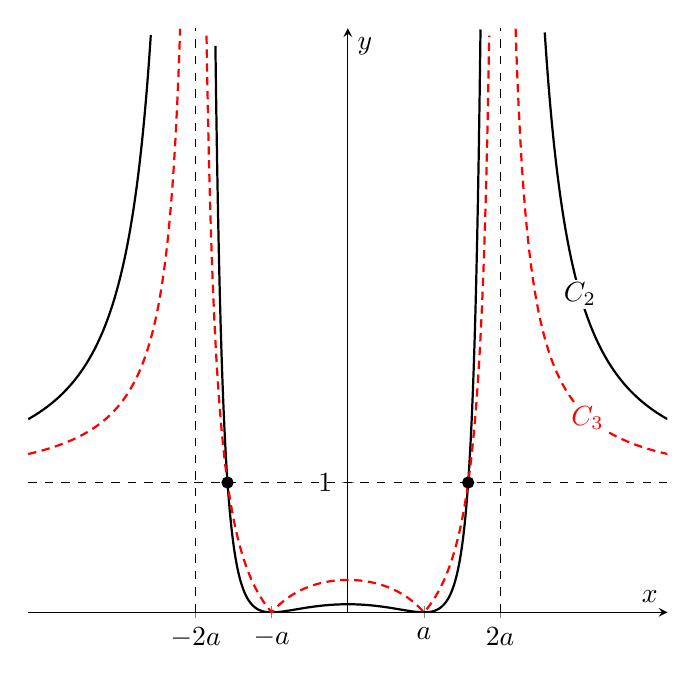
\begin{tikzpicture}
\begin{axis}[
  axis lines=middle,
  width=0.8\linewidth,
  height=9cm,
  xmin=-4.2, xmax=4.2,
  ymin=0, ymax=4.5,
  xtick={-2,-1,1,2},
  xticklabels={$-2a$,$-a$,$a$,$2a$},
  ytick={1},
  yticklabels={$1$},
  xlabel={$x$},
  ylabel={$y$},
  samples=350,
  clip=true,
  restrict y to domain=0:4.5,
  unbounded coords=jump
]
  \addplot[dashed, domain=-4.2:4.2] {1};
  \addplot[dashed] coordinates {(-2,0) (-2,4.5)};
  \addplot[dashed] coordinates {(2,0) (2,4.5)};
  \addplot[thick, domain=-4.2:-2.03] {((x^2-1)/(x^2-4))^2};
  \addplot[thick, domain=-1.99:1.97] {((x^2-1)/(x^2-4))^2};
  \addplot[thick, domain=2.01:4.2] {((x^2-1)/(x^2-4))^2};
\addplot[thick, densely dashed, red, domain=-4.2:-2.03] {abs((x^2-1)/(x^2-4))};
\addplot[thick, densely dashed, red, domain=-1.97:1.97] {abs((x^2-1)/(x^2-4))};
\addplot[thick, densely dashed, red, domain=2.03:4.2] {abs((x^2-1)/(x^2-4))};
\node[text=red, fill=white, inner sep=1pt] at (axis cs:3.15,1.5) {$C_3$};
  \addplot[only marks, mark=*] coordinates {
    (-1.5811,1) (1.5811,1)
  };
  \node[fill=white, inner sep=1pt] at (axis cs:3.05,2.45) {$C_2$};
\end{axis}
\end{tikzpicture}} & & \\
& \msFeature{Shape} & B1 & {\(C_2\): on or above the \(x\)-axis, touching at \((\pm a,0)\), maximum on the \(y\)-axis, asymptotes \(x=\pm2a\) and \(y=1\), outer branches above \(y=1\).} \\
& \msFeature{Shape} & B1 & {\(C_3\): \(C_1\) with parts below the \(x\)-axis reflected, cusps at \((\pm a,0)\), same asymptotes.} \\
& \msFeature{Labelled point} & B1 & {Curves labelled, meeting at \((\pm a,0)\) and crossing on \(y=1\); \(C_2\) below \(C_3\) between the crossings, above outside them.} \\
& {Critical values \(x = \pm a\sqrt{\tfrac52}\)} & M1 & {Uses their \(x\)-coordinates of the intersections on \(y=1\) as the ends of the interval.} \\
& {\(-a\sqrt{\tfrac52} \leq x \leq a\sqrt{\tfrac52}\)} & A1 & {oe, including set notation. A0 for strict inequalities or extra intervals.} \\
\nopagebreak & & [5] & \\
\nopagebreak \SetCell[c=2]{r} Total for Question 14 & & 14 & \\
\end{msscheme}

\end{document}
